\documentclass{article}
\usepackage{amsthm}
\newtheorem{definition}{Definition}
\newtheorem{theorem}{Theorem}

\usepackage{graphicx}
\usepackage{float}

\title{unit test and refactoring, ideas collected for personal usage}
\date{2022-06-18}
\author{Florin Ioan Chertes}

\begin{document}

\maketitle
\pagenumbering{gobble}
\newpage
\pagenumbering{arabic}


\begin{abstract}
Unit test and refactoring are processes that go hand in hand with the purpose fostering the creation of high source code quality. These both processes make the maintainability of the source code manageable and prepare it for reliable change.
\end{abstract}

\section{Introduction}

As Beck \cite{BecAnd04extreme, beck2001planning} explains, testing is one of the most important parts of the discipline Extreme Programming (\textit{XP}). In his view development is driven by tests, you test first, then you code. When all the tests run, and you can't think of any more tests that would break, you are done adding functionality. He mentions the importance of integration tests that follow immediately the development. Automated test give the possibility to defer the important design decisions as late as possible when the requirements are better understood. Feedback is one of the most important values of XP. Feedback works at different time scales. The programmers write unit tests for all the logic in program that could break. The customers write stories (description of features, simplified use-cases). The testers write functional testes, business functionality for all stories. So the unit tests, written by developers and the functional tests written by customers and testers are the hard of the \textit{XP}.   

\section{Unit Test}

\subsection{Unit Test in Detail}

Feather \cite{FeathersMichael} says that the concept of unit test is about the idea that they are tests in isolation of individual software components. But what are components? The definition could vary, but in unit tests we are usually concerned with the most atomic behavioral units of the system. In object oriented code the units are the classes.


\subsection{Modern \textit{unit test} concepts}

Khorikov \cite{Khoricov2020} introduced the \textit{unit test} based on the work of many practitioners and scholars for more than a quarter of century.

\begin{definition}
\begin{itemize}
Unit tests are automatic tests having the following properties:
	\item a unit test verifies a single unit of behavior,
	\item does it quickly and
	\item does it in isolation from other tests.
\end{itemize}
\end{definition}


The \textit{isolation issue} is the most disputed. The dispute led to the formation of two schools of unit testing: the classical (Detroit) school, and the London (\textit{mockist}) school. This difference of opinion affects the view of what constitutes a unit and the treatment of the system under test’s (\textit{SUT}’s) dependencies.

\begin{itemize}
	\item The London school states that \textit{the units under test} should be isolated from each other. A unit under test is a unit of code, usually a class. All of its dependencies, except immutable dependencies, should be replaced with test doubles in tests.
	\item The classical school states that \textit{the unit tests} need to be isolated from each other, not \textit{the units under test}. Also, \textit{a unit under test} is a unit of behavior, not a unit of code. Thus, only shared dependencies should be replaced with test doubles. Shared dependencies are dependencies that provide means for tests to affect each others execution flow.
\end{itemize}

The London school provides the benefits of better granularity, the ease of testing large graphs of interconnected classes, and the ease of finding which functionality contains a bug after a test failure.

The benefits of the London school look appealing at first. However, they introduce several issues. \textit{First}, the focus on classes under test is misplaced: tests should verify units of behavior, not units of code. \textit{Furthermore}, the inability to unit test a piece of code is a strong sign of a problem with the code design. The use of test doubles doesn’t fix this problem, but rather only hides it. And \textit{finally}, while the ease of determining which functionality contains a bug after a test failure is helpful, it’s not that big a deal because you often know what caused the bug anyway—it’s what you edited last.

The biggest issue with the London school of unit testing is the problem of over specification—coupling tests to the \textit{SUT}’s implementation details.

\begin{definition}
An integration test is a test that doesn’t meet at least one of the criteria for a unit test. 
\end{definition}

\begin{definition}
End-to-end tests are a subset of integration tests; they verify the system from the end user’s point of view. End-to-end tests reach out directly to all or almost all out-of-process dependencies your application works with.
\end{definition}


\subsection{Are the classes or the modules the support of the behavior?}

The Test-driven design \cite{beck2002driven} was wrong understood and used, says Cooper \cite{WEBSITE:WhereDidItAllGoWrong}. Heinemeier Hansson \cite{WEBSITE:TDDisdead} even says that \textit{TDD} is dead. They both go back to the roots of \textit{TDD} and agree that: 

\begin{itemize}
	\item test behavior, this is the stable contract of the \textit{API}, 
	\item do not test implementation details, these details can change very rapidly
	\item test the implementation details only when you need to understand the refactoring of the implementation, afterwords delete these tests.
\end{itemize}

The common \textit{TDD} practice by using: 'adding a new method to a class' as the trigger to write a test, is simply wrong. Adding a new class is not the trigger for writing tests. The trigger is implementing a requirement.
The stable part of the implementation is its public exposed API of the module, this must be tested. Write test to cover the use cases or stories, use the model: \textit{Given}, \textit{When}, \textit{Then}. The subject under test (\textit{SUT}) is not a class, \textit{SUT} is the export from a module, its facade.
Unit means a module not a class, modules consist of many classes that constitute the implementation detail.

In Beck \cite{beck2002driven}, is explained, that the object of \textit{TDD} is to test behavior in the system. When it runs in isolation, is the test not a class using mocks to be isolated. The test is isolated not the \textit{SUT}.
The test are:
\begin{itemize}
	\item unit test of the module,
	\item integration test and
	\item system test.
\end{itemize}

If is it difficult to use file system, database, etc., in the unit tests, do not mock them, but fixtures to put your unit tests to use the file system, database, etc. Writing tests that target a method on a class, is not a \textit{TDD} developer test. \textit{TDD} unit tests focus on a story, use-case, scenario, etc. Unit test focusing on method are hard to maintain, these tests do not capture the behavior they want to preserve, detail implementation exposed to unit tests make refactoring difficult. In the \textit{TDD} cycle when you are ready with the implementation, you do not write new unit tests, when refactoring to clean code.

Eliminate the dependency between tests an production code. Tests must not depend on implementation details, because changing the implementation, breaks the tests. Tests must depend on contracts, or public interfaces. This allows for refactor implementation without changing tests. Do not test implementation details, they change quickly. Do not use mocks to confirm implementation details.

Coplien \cite{WEBSITE:UnitTestIsWaste} considers unit tests a waste. He consider to automate:
\begin{itemize}
	\item integration tests, 
	\item bug regression tests and 
	\item system tests 
\end{itemize}
rather than automating unit tests. 

A smarter approach would reduce the test code mass through formal test design: that is, to do formal boundary-condition checking, more white-box testing, and so forth. That requires that the unit under test be designed for test-ability. This is how hardware engineers do it: designers provide "test points" that can read out values on a J-Tag pin of a chip, to access internal signal values of the chip — tantamount to accessing values between intermediate computations in a computational unit. I advocate doing this at the system level where the testing focus should lie; I have never seen anyone achieve this at the unit level. Without such hooks you are limited to black-box unit testing. 

Tests should be designed with great care. Business people, rather than programmers, should design most functional tests. Unit tests should be limited to those that can be held up against some “third-party” success criteria.

In Coplien \cite{WEBSITE:UnitTestIsWaste} we find the description of a project in which the developers had written their tests in such a way, that they didn't have to change the tests when the functionality changed. That of course means that the tests  weren't testing the functionality, so whatever they were testing was of little value. Those have no provable value. There were methodologies in the 1970s and 1980s based on trace-ability that tried to reduce system requirements all the way down to the unit level. In general, that's an NP-hard problem (unless you are doing pure procedural decomposition) so I'm very skeptical of anyone who says they can do that. So one question to ask about every test is: If this test fails, what business requirement is compromised? Most of the time, the answer is, "I don't know." If you don't know the value of the test, then the test theoretically could have zero business value. The test does have a cost: maintenance, computing time, administration, and so forth. That means the test could have net negative value. That is the fourth category of tests to remove. These are tests which, though they may even do some amount of verification, do no validation.

In summary: 
\begin{itemize}
	\item Keep regression tests around for up to a year — but most of those will be system-level tests rather than unit tests. 
	\item Keep unit tests that test key algorithms for which there is a broad, formal, independent oracle of correctness, and for which there is ascribable business value.
	\item  Except for the preceding case, if X has business value and you can test X with either a system test or a unit test, use a system test — context is everything.
	\item Design a test with more care than you design the code.
	\item Turn most unit tests into assertions.
	\item Throw away tests that haven’t failed in a year.
	\item Testing can’t replace good development: a high test failure 
rate suggests you should shorten development intervals, 
perhaps radically, and make sure your architecture and design 
regimens have teeth
	\item If you find that individual functions being tested are trivial, 
double-check the way you incentivize developers’ 
performance. Rewarding coverage or other meaningless 
metrics can lead to rapid architecture decay.
	\item Be humble about what tests can achieve. Tests don’t improve 
quality: developers do
\end{itemize}

\subsection{\textit{TDD} and Software Design Quality}

Test-driven development (\textit{TDD}) creates software \cite{TestDrivenDevelopmentConceptsTaxonomy} in very short iterations with minimal upfront design. Poised for widespread adoption, \textit{TDD} has become the focus of an increasing number of researchers and developers.

Support for test-driven development, \textit{TDD} is growing in many development contexts beyond its common association with extreme programming.  We \cite{TestDrivenDevelopmentReallyImproveSoftwareDesign} weren't able to confirm claims that\textit{TDD} improves cohesion while lowering coupling, but we anticipate ways to clarify the questions these design characteristics raised. In particular, we're working to eliminate the confounding factor of accessor usage in the cohesion metrics.

It is suggested \cite{DoesTestDrivenDevelopmentImprovetheProgramCode} that test-driven development, \textit{TDD} is one of the most fundamental practices in agile software development, which produces loosely coupled and highly cohesive code. However, how the \textit{TDD} impacts on the structure of the program code have not been widely studied. This paper presents the results from a comparative case study of five small scale software development projects where the effect of \textit{TDD} on program design was studied using both traditional and package level metrics. The empirical results reveal that an unwanted side effect can be that some parts of the code may deteriorate. In addition, the differences in the program code, between \textit{TDD} and the iterative test-last development, were not as clear as expected. This raises the question as to whether the possible benefits of \textit{TDD} are greater than the possible downsides. Moreover, it additionally questions whether the same benefits could be achieved just by emphasizing unit-level testing activities.

\section{The goal of unit testing }

In Khorikov \cite{Khoricov2020} we find that, learning unit testing doesn’t stop at mastering the technical bits of it, such as your favorite test framework, mocking library, and so on. There’s much more to unit testing than the act of writing tests. You always have to strive to achieve the
best return on the time you invest in unit testing, minimizing the effort you put into tests and maximizing the benefits they provide. Achieving both things isn’t an easy task.

\subsection{The current state of unit testing}
For the past two decades, there’s been a push toward adopting unit testing. The push has been so successful that unit testing is now considered mandatory in most companies. Most programmers practice unit testing and understand its importance. There’s no longer any dispute as to whether you should do it. Unless you’re working on a throwaway project, the answer is, yes, you do.

\subsection{The goal of unit testing}
The goal is to enable sustainable growth of the software project. The term sustainable is key. It’s quite easy to grow a project, especially when you start from scratch. It’s much harder to sustain this growth over time.

In software, entropy manifests in the form of code that tends to deteriorate. Each time you change something in a code base, the amount of disorder in it, or entropy, increases. If left without proper care, such as constant cleaning and refactoring, the system becomes increasingly complex and disorganized. Fixing one bug introduces more bugs, and modifying one part of the software breaks several others—it’s like a domino effect. Eventually, the code base becomes unreliable. And worst of all, it’s hard to bring it back to stability.

\begin{definition}
A \textbf{regression} \cite{regression_testing_in_practice} is when a feature stops working as intended after a certain event (usually, a code modification). The terms \textbf{regression} and \textbf{software bug} are synonyms and can be used interchangeably.
\end{definition}


\subsection{Using coverage metrics to measure test suite quality}


\subsection{What makes a good or bad test?}
Although unit testing helps maintain project growth, it’s not enough to just write tests. 
Remember, \textit{not all tests are created equal}. Some of them are valuable and contribute a lot to overall software quality. Others don’t. They raise false alarms, don’t help you catch regression errors, and are slow and difficult to maintain. It’s easy to fall into the trap of writing unit tests for the sake of unit testing without a clear picture of whether it
helps the project.

\subsubsection{Production code vs. test code}
People often think production code and test code are different. Tests are assumed to be an addition to production code and have no cost of ownership. By extension, people often believe that the more tests, the better. This isn’t the case. \textbf{Code is a liability, not an asset}. The more code you introduce, the more you extend the surface area for potential bugs in your software, and the higher the project’s upkeep cost. It’s always better to solve problems with as little code as possible. Tests are code, too. You should view them as the part of your code base that aims at solving a particular problem: ensuring the application’s correctness. \textbf{Unit tests, just like any other code, are also vulnerable to bugs and require maintenance}.

\subsection{What makes a successful test suite?}

\begin{definition}
A successful test suite has the following properties:
\begin{itemize}
	\item It’s integrated into the development cycle.
	\item It targets only the most important parts of your code base.
	\item It provides maximum value with minimum maintenance costs.
\end{itemize}
\end{definition}

 It’s important to \textbf{direct your unit testing efforts to the most critical parts of the system} and verify the others only briefly or indirectly. In most applications, the most important part is the part that contains business logic—the \textit{domain model}, Evans \cite{evans2004} .  Testing business logic gives you the best return on your time investment.

\subsection{It provides maximum value with minimum maintenance costs}
The most difficult part of unit testing is achieving maximum value with minimum maintenance costs.
It’s not enough to incorporate tests into a build system, and it’s not enough to maintain high test coverage of the domain model. It’s also crucial to keep in the suite only the tests whose value exceeds their upkeep costs by a good margin.

This last attribute can be divided in two:
\begin{itemize}
	\item Recognizing a valuable test (and, by extension, a test of low value)
	\item Writing a valuable test
\end{itemize}

Although these skills may seem similar, they’re different by nature. To recognize a test of high value, you need a frame of reference. On the other hand, writing a valuable test requires you to also know code design techniques. Unit tests and the underlying code are highly intertwined, and it’s impossible to create valuable tests without putting significant effort into the code base they cover. 

You can view it as the difference between recognizing a good song and being able to compose one. The amount of effort required to become a composer is asymmetrically larger than the effort required to differentiate between good and bad music. The same is true for unit tests. Writing a new test requires more effort than examining an existing one, mostly because you don’t write tests in a vacuum: you have to take into account the underlying code.

\section{What is a unit test?}

\subsection{The definition of “unit test”}

\begin{definition}
\begin{itemize}
Unit tests are automatic tests having the following properties:
	\item a unit test verifies a single unit of behavior,
	\item does it quickly and
	\item does it in isolation from other tests.
\end{itemize}
\end{definition}

What people have vastly different opinions about is the third attribute. The isolation issue is the root of the differences between the \textit{classical}, Detroit and London, \textit{mockist} schools of
unit testing.

\subsubsection{The isolation issue: The London take}

What does it mean to verify a piece of code—a unit—in an isolated manner? The London school describes it as isolating the system under test from its collaborators. It means if a class has a dependency on another class, or several classes, you need to replace all such dependencies with test \textit{doubles}. This way, you can focus on the class under test exclusively by separating its behavior from any external influence.

\begin{definition}
A \textbf{test double} is an object that looks and behaves like its release-intended counterpart but is actually a simplified version that reduces the complexity and facilitates testing. This term was introduced by Meszaros \cite{Meszaros07}. The name itself comes from the notion of a stunt double in movies.
\end{definition}

One benefit of this approach is that if the test fails, you know for sure which part of the code base is broken: it’s the system under test. There could be no other suspects, because all of the class’s neighbors are replaced with the test doubles.

Another benefit is the ability to split the object graph—the web of communicating classes solving the same problem. This web may become quite complicated: every class in it may have several immediate dependencies, each of which relies on dependencies of their own, and so on. Classes may even introduce circular dependencies, where the chain of dependency eventually comes back to where it started.

With test doubles, you can put a stop to this. You can substitute the immediate dependencies of a class; and, by extension, you don’t have to deal with the dependencies of those dependencies, and so on down the recursion path. You are effectively breaking up the graph—and that can significantly reduce the amount of preparations you have to do in a unit test.

\begin{definition}
A mock is a special kind of test double that allows you to examine interactions between the system under test and its collaborators.
\end{definition}

\subsubsection{The isolation issue: The classical take}
How small should a small piece of code be? As you saw from the previous section, if you adopt the position of isolating every individual class, then it’s natural to accept that the piece of code under test should also be a single class, or a method inside that class. 

In the classical approach, it’s not the code that needs to be tested in an isolated manner. Instead, unit tests themselves should be run in isolation from each other. That way, you can run the tests in parallel, sequentially, and in any order, whatever fits you best, and they still won’t affect each others outcome.

Isolating tests from each other means it’s fine to exercise several classes at once as long as they all reside in the memory and don’t reach out to a shared state, through which the tests can communicate and affect each others execution context. Typical examples of such a shared state are out-of-process dependencies—the database, the file system, and so on.

\begin{definition}
A \textbf{shared dependency} is a dependency that is shared between tests and provides means for those tests to affect each others outcome. 
\begin{itemize}
	\item A typical example of shared dependencies is a static mutable field. A change to such a field is visible across all unit tests running within the same process. 
	\item A database is another typical example of a shared dependency.
\end{itemize}
\end{definition}

\begin{definition}
A \textbf{private dependency} is a dependency that is not shared.
\end{definition}

\begin{definition}
An \textbf{out-of-process dependency} is a dependency that runs outside the application’s execution process; it’s a proxy to data that is not yet in the memory. 
\end{definition}

 An out-of-process dependency corresponds to a shared dependency in the vast majority of cases, but not always. For example, a database is both out-of-process and shared. But if you launch that database in a Docker container before each test run, that would make this dependency out-of-process but not shared, since tests no longer work with the same instance of it. Similarly, a read-only database is also out-of-process but not shared, even if it’s reused by tests. Tests can’t mutate data in such a database and thus can’t affect each others outcome.

Note that shared dependencies are shared between unit tests, not \textit{between} classes under test (units). In that sense, a \textbf{singleton dependency} is not shared as long as you are able to create a new instance of it in each test. While there’s only one instance of a singleton in the production code, tests may very well not follow this pattern and not reuse that singleton. Thus, such a dependency would be private.

You can't create a new file system or a database, however; they must be either
\begin{itemize}
	\item shared between tests or
	\item substituted away with test doubles.
\end{itemize}

Another reason for substituting shared dependencies is to increase the test execution speed.

\subsection{The classical and London schools of unit testing}

 The London school views it as isolation of the system under test from its collaborators, whereas the classical school views it as isolation of unit tests themselves from each other.  This seemingly minor difference has led to a vast disagreement about how to approach unit testing, which, as you already know, produced the two schools of thought. Overall, the disagreement between the schools spans three major topics:
\begin{itemize}
	\item The isolation requirement
	\item What constitutes a piece of code under test (a unit)
	\item Handling dependencies
\end{itemize}

 In real-world projects, you rarely have a shared dependency that isn't out-of-process. If a dependency is in-process, you can easily supply a separate instance of it to each test; there’s no need to share it between tests. Similarly, you normally don't encounter an out-of-process dependency that’s not shared. Most such dependencies are mutable and thus can be
modified by tests.

\subsection{ Contrasting the classical and London schools of unit testing}

The classical school of unit testing tends to produce tests of higher quality and thus is better suited for achieving the ultimate goal of unit testing, which is the sustainable growth of your project. The reason is fragility: tests that use \textbf{mocks} tend to be more brittle than classical tests. For now, let’s take the main selling points of the London school and evaluate them one by one. The London school’s approach provides the following benefits:
\begin{itemize}
	\item \textit{Better granularity.} The tests are fine-grained and check only one class at a time.
	\item \textit{It’s easier to unit test a larger graph of interconnected classes.} Since all collaborators
are replaced by test doubles, you don’t need to worry about them at the time of
writing the test.
	\item \textit{If a test fails, you know for sure which functionality has failed.} Without the class’s collaborators, there could be no suspects other than the class under test itself. Of course, there may still be situations where the system under test uses a value object and it’s the change in this value object that makes the test fail. But these cases aren’t that frequent because all other dependencies are eliminated in tests.
\end{itemize}

\subsubsection{ Unit testing one class at a time}
The point about better granularity relates to the discussion about what constitutes a unit in unit testing. The London school considers a class as such a unit. Coming from an object-oriented programming background, developers usually regard classes as the atomic building blocks that lie at the foundation of every code base. This naturally leads to treating classes as the atomic units to be verified in tests, too. This tendency is understandable but misleading.

Tests shouldn’t verify \textit{units of code}. Rather, they should verify \textit{units of behavior}: something that is meaningful for the problem domain and, ideally, something that a business person can recognize as useful. The number of classes it takes to implement such a unit of behavior is irrelevant. The unit could span across multiple classes or only one class, or even take up just a tiny method.

And so, aiming at better code granularity isn’t helpful. As long as the test checks a single unit of behavior, it’s a good test. Targeting something less than that can in fact damage your unit tests, as it becomes harder to understand exactly what these tests verify. \textit{A test should tell a story about the problem your code helps to solve, and this story should be cohesive and meaningful to a non-programmer.}

\subsubsection{Unit testing a large graph of interconnected classes}

The use of mocks in place of real collaborators can make it easier to test a class - especially when there’s a complicated dependency graph, where the class under test has dependencies, each of which relies on dependencies of its own, and so on, several layers deep. With test doubles, you can substitute the class’s immediate dependencies and thus break up the graph, which can significantly reduce the amount of preparation you have to do in a unit test. If you follow the classical school, you have to re-create the full object graph (with the exception of shared dependencies) just for the sake of setting up the system under test, which can be a lot of work.

Although this is all true, this line of reasoning focuses on the wrong problem. Instead of finding ways to test a large, complicated graph of interconnected classes, you should focus on not having such a graph of classes in the first place. More often than not, a large class graph is a result of a code design problem.

The use of mocks only hides this problem; it doesn’t tackle the root cause. 

\subsubsection{Revealing the precise bug location}
If you introduce a bug to a system with London-style tests, it normally causes only tests whose \textit{SUT} contains the bug to fail. However, with the classical approach, tests that target the clients of the malfunctioning class can also fail. This leads to a ripple effect where a single bug can cause test failures across the whole system. As a result, it becomes harder to find the root of the issue. You might need to spend some time debugging the tests to figure it out.

\begin{theorem}
If you run your tests regularly (ideally, after each source code change), then you know what caused the bug — it’s what you edited last, so it’s not that difficult to find the issue. Also, you don’t have to look at all the failing tests. Fixing one automatically fixes all the others.
\end{theorem}

\begin{theorem}
There’s value in failures cascading all over the test suite. If a bug leads to a fault in not only one test but a whole lot of them, it shows that the piece of code you have just broken is of great value — the entire system depends on it. That’s useful information to keep in mind when working with the code.
\end{theorem}

The London style of unit testing leads to outside-in TDD, where you start from the higher-level tests that set expectations for the whole system. By using mocks, you specify which collaborators the system should communicate with to achieve the expected result. You then work your way through the graph of classes until you implement every one of them. 

The classical school doesn’t provide quite the same guidance since you have to deal with the real objects in tests. Instead, you normally use the inside-out approach. In this style, you start from the domain model and then put additional layers on top of it until the software becomes usable by the end user.

But the most crucial distinction between the schools is the issue of over-specification: that is, coupling the tests to the \textit{SUT}’s implementation details. The London style tends to produce \textbf{tests that couple to the implementation} more often than the classical style. And this is the main objection against the ubiquitous use of mocks and the London style in general.

\subsection{Integration tests in the two schools}

\begin{definition}
A test is an integration test when it verifies two or more units of behavior. An integration test can also verify how two or more modules developed by separate teams work together. 
\end{definition}

\subsubsection{ End-to-end tests are a subset of integration tests}

\begin{definition}
An integration test is a test that verifies that your code works in integration with shared dependencies, out-of-process dependencies, or code developed by other teams in the organization.
\end{definition}

\begin{definition}
End-to-end tests are a subset of integration tests. They, too, check to see how your code works with out-of-process dependencies. The difference between an end-to-end test and an integration test is that end-to-end tests usually include more of such dependencies.
\end{definition}

\section{The four pillars of a good unit test}

\subsection{Diving into the four pillars of a good unit test}

A good unit test has the following four attributes:
\begin{itemize}
	\item Protection against regressions
	\item Resistance to refactoring
	\item Fast feedback
	\item Maintainability
\end{itemize}

\subsubsection{The first pillar: Protection against regressions}

\begin{definition}
A \textbf{regression} \cite{regression_testing_in_practice} is a software bug. It’s when a feature stops working as intended after some code modification, usually after you roll out new functionality.
\end{definition}

\begin{theorem}
An unfortunate fact of programming life is that \textbf{code is not an asset, it’s a liability}. The larger the code base, the more exposure it has to potential bugs.
\end{theorem}

To evaluate how well a test scores on the metric of protecting against regressions, you need to take into account the following:
\begin{itemize}
	\item The amount of code that is executed during the test
	\item The complexity of that code
	\item The code’s domain significance
\end{itemize}	
Generally, the larger the amount of code that gets executed, the higher the chance that the test will reveal a regression. 
Code that represents complex business logic is more important than boilerplate code—bugs in business-critical functionality are the most damaging. It’s rarely worthwhile to test trivial code. Such code is short and doesn’t contain a substantial amount of business logic. Tests that cover trivial code don’t have much of a chance of finding a regression error, because there’s not a lot of room for a mistake.

\begin{theorem}
To maximize the metric of protection against regressions, the test needs to aim at exercising as much code as possible. 
\end{theorem}

\subsubsection{The second pillar: Resistance to refactoring}
\begin{definition}
\textbf{resistance to refactoring} is the degree to which a test can sustain a refactoring of the underlying application code without turning red (failing).
\end{definition}

A \textit{false positive} is a false alarm. This situation occurs when after refactoring everything looks even better than before, but the test is failing. You look more closely to see exactly what you broke with the refactoring, but it turns out that you didn’t break anything. The feature works perfectly, just as before. The problem is that the tests are written in such a way that they turn red with any modification of the underlying code. And they do that regardless of whether you actually break the functionality itself.

Such false positives usually take place when you refactor the code—when you modify the implementation, but keep the observable behavior intact. Hence the name for this attribute of a good unit test: \textit{resistance to refactoring}.

\subsubsection{What causes false positives?}
The number of false positives a test produces is directly related to the way the test is structured. The more the test is coupled to the implementation details of the system under test (\textit{SUT}), the more false alarms it generates.  

\begin{theorem}
The only way to reduce the chance of getting a false positive is to decouple the test from those implementation details. You need to make sure the test verifies the end result the \textit{SUT} delivers: its \textbf{observable behavior, not the steps} it takes to do that.
\end{theorem}

\subsection{The intrinsic connection between the first two attributes}
There’s an intrinsic connection between the first two pillars of a good unit test:

\begin{itemize}
	\item \textit{protection against regressions} and 
	\item \textit{resistance to refactoring}.
\end{itemize}	

They both contribute to the accuracy of the test suite, though from opposite perspectives. These two attributes also tend to influence the project differently over time: while it’s important to have good protection against regressions very soon after the project’s initiation, the need for resistance to refactoring is not immediate.

When the test doesn’t catch an error, that’s a problem, a \textit{false negative}. And this is what the first attribute of a good test—\textit{protection against regressions}—helps you avoid. Tests with a good \textit{protection against regressions} help you to minimize the number of false negatives.

On the other hand, there’s a symmetric situation when the functionality is correct but the test still shows a failure. This is a \textit{false positive}, a false alarm. And this is what the second attribute—\textit{resistance to refactoring}—helps you with.

The accuracy metric itself consists of two components:

\begin{itemize}
	\item How good the test is at indicating the presence of bugs (lack of false negatives, the sphere of \textit{protection against regressions}) 
	\item How good the test is at indicating the absence of bugs (lack of false positives, the sphere of \textit{resistance to refactoring})
\end{itemize}	

\begin{theorem}
In order to be valuable, the test needs to score at least something in all four categories.
\end{theorem}

Remember, all code, including test code, is a liability. Set a fairly high threshold for the minimum required value, and only allow tests in the suite if they meet this threshold. A small number of highly valuable tests will do a much better job sustaining project growth than a large number of mediocre tests.

End-to-end tests exercise a lot of code, they provide the best protection against regressions.

End-to-end tests are also immune to false positives and thus have a good resistance to refactoring.

However, despite these benefits, end-to-end tests have a major drawback: they are slow. Any system that relies solely on such tests would have a hard time getting rapid feedback. 

\section{Mocks and test fragility}

The use of mocks in tests is a controversial subject. Some people argue that mocks are a great tool and apply them in most of their tests. Others claim that mocks lead to test fragility and try not to use them at all. As the saying goes, the truth lies somewhere in between. Mocks often result in fragile tests—tests that lack the metric of resistance to refactoring. But there are still cases where mocking is applicable and even preferable.

\subsection{Differentiating mocks from stubs}

There are two types of test doubles, that that allows for examine interactions between the system under test (\textit{SUT}) and its collaborators. : \textit{mocks} and \textit{stubs}.

\subsubsection{The types of test doubles}

According to Gerard Meszaros, there are five variations of test doubles: \textit{dummy, stub, spy, mock, and fake}. Such a variety can look intimidating, but in reality, they can all be grouped together into just two types: mocks and stubs.

The difference between these two types boils down to the following: 
\begin{itemize}
	\item Mocks help to emulate and examine outcoming interactions. These interactions are calls the SUT makes to its dependencies to change their state.
	\item Stubs help to emulate incoming interactions. These interactions are calls the SUT makes to its dependencies to get input data.
\end{itemize}

\begin{theorem}
Asserting interactions with stubs is a common anti-pattern that leads to fragile tests.
\end{theorem}

The only way to avoid false positives and thus improve resistance to refactoring in tests is to make those tests verify the end result (which, ideally, should be meaningful to a non-programmer), not implementation details.

\subsubsection{How mocks and stubs relate to commands and queries}

Test doubles that substitute commands become mocks. Similarly, test doubles that substitute queries are stubs. 

\subsection{Observable behavior vs. implementation details}
The metric of resistance to refactoring is the most important because whether a unit test possesses this metric is mostly a binary choice. 

The main reason tests deliver false positives (and thus fail at resistance to refactoring) is because they couple to the code’s implementation details. The only way to avoid such coupling is to verify the end result the code produces (its observable behavior) and distance tests from implementation details as much as possible. In other words, tests must focus on the \textit{whats}, not the \textit{hows}. So, what exactly is an implementation detail, and how is it different from an observable behavior?

For a piece of code to be part of the system’s observable behavior, it has to do one of the following things:

\begin{itemize}
	\item Expose an operation that helps the client achieve one of its goals. An operation is
a method that performs a calculation or incurs a side effect or both.
	\item Expose a state that helps the client achieve one of its goals. State is the current
condition of the system.
\end{itemize}

Ideally, the system’s public API surface should coincide with its observable behavior, and all its implementation details should be hidden from the eyes of the clients. Such a system has a well-designed API

\subsection{The classical vs. London schools of unit testing, revisited}

The indiscriminate use of mocks is why following the London school often results
in tests that couple to implementation details and thus lack resistance to refactoring.
The metric of resistance to refactoring (unlike the other three) is mostly a binary choice: a test either has resistance to refactoring or it doesn’t. Compromising on this metric renders the test nearly worthless.

\section{Styles of unit testing}

\subsection{The three styles of unit testing}


There are three such \textit{unit test styles}:
\begin{itemize}
	\item output-based,
	\item state-based and
	\item	 communication based testing.
\end{itemize}
Among the three, the \textit{output-based} style produces tests of the highest
quality, \textit{state-based} testing is the second-best choice, and \textit{communication-based}
testing should be used only occasionally.

\subsubsection{Defining the output-based style}

\begin{definition}
The \textbf{output-based} style, where you feed an input to the system under test (SUT) and check the output it produces. This style of unit testing is only applicable to code that doesn’t change a global or internal state, so the only component to verify is its return value.
\end{definition}

\begin{definition}
The \textit{output-based} style of unit testing is also known as \textbf{functional}.
\end{definition}


\subsubsection{Defining the state-based style}

\begin{definition}
The \textbf{state-based} style is about verifying the state of the system after an operation is complete. The term state in this style of testing can refer to the state of the SUT itself, of one of its collaborators, or of an out-of-process dependency, such as the database or the file-system.
\end{definition}

\subsubsection{Defining the communication-based style}

\begin{definition}
The  style of unit testing called \textbf{communication-based} testing uses mocks to verify communications between the system under test and its collaborators.
\end{definition}

\subsection{Comparing the three styles of unit testing}
\subsubsection{Comparing the styles using the metrics of protection against regressions and feedback speed}

The metric of protection against regressions doesn’t depend on a particular style of testing. This metric is a product of the following three characteristics:
\begin{itemize}
	\item the amount of code that is executed during the test,
	\item the complexity of that code and
	\item	 its domain significance.
\end{itemize}
Generally, you can write a test that exercises as much or as little code as you like; no particular style provides a benefit in this area. The same is true for the code’s complexity and domain significance.

The only exception is the communication-based style: overusing it can result in shallow tests that verify only a thin slice of code and mock out everything else. Such shallowness is not a definitive feature of communication based testing, though, but rather is an extreme case of abusing this technique.

\subsubsection{Comparing the styles using the metric of resistance to refactoring}

When it comes to the metric of resistance to refactoring, the situation is different. Resistance to refactoring is the measure of how many false positives (false alarms) tests generate during refactorings. False positives, in turn, are a result of tests coupling to code’s implementation details as opposed to observable behavior.

\begin{theorem}
\textit{Output-based testing} provides the best protection against false positives because the resulting tests couple only to the method under test. The only way for such tests to couple to implementation details is when the method under test is itself an implementation detail.
\end{theorem}

State-based testing is usually more prone to false positives.  Communication-based testing is the most vulnerable to false alarms.

Mocks are fine only when they verify interactions that cross the application boundary and only when the side effects of those interactions are visible to the external world.

You can reduce the number of false positives to a minimum by maintaining proper encapsulation and coupling tests to observable behavior only.

\section{Refactoring toward valuable unit tests}

\subsection{Identifying the code to refactor}
It’s rarely possible to significantly improve a test suite without refactoring the underlying code. There’s no way around it—test and production code are intrinsically connected.

\subsubsection{The four types of code}
All production code can be categorized along two dimensions:
\begin{itemize}
	\item complexity or domain significance and
	\item the number of collaborators.
\end{itemize}

\begin{definition}
\textbf{Code complexity} is defined by the number of decision-making (branching) points in the code. The greater that number, the higher the complexity.
\end{definition}

\begin{definition}
\textbf{Domain significance} shows how significant the code is for the problem domain of your project. Normally, all code in the domain layer has a direct connection to the end users’ goals and thus exhibits a high domain significance. On the other hand, utility code doesn’t have such a connection.
\end{definition}

Complex code and code that has domain significance benefit from unit testing the most because the corresponding tests have great protection against regressions.

The second dimension is the number of collaborators a class or a method has. A collaborator is a dependency that is either mutable or out-of-process (or both). Code with a large number of collaborators is expensive to test. That’s due to the maintainability metric, which depends on the size of the test. It takes space to bring collaborators to an expected condition and then check their state or interactions with them afterward. And the more collaborators there are, the larger the test becomes.

Use mocks to verify interactions that cross the application boundary in order to maintain proper resistance to refactoring. 

The combination of code complexity, its domain significance, and the number of collaborators give us the four types of code:
\begin{itemize}
	\item domain model and algorithms,
	\item trivial code,
	\item controllers and
	\item over complicated code.	
\end{itemize}

\begin{figure}[H]
  \centering
  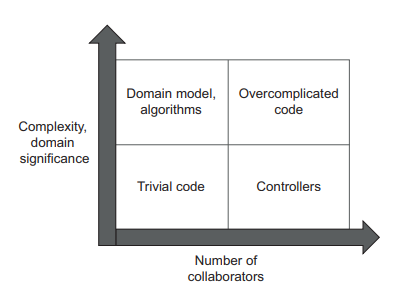
\includegraphics[width=1.0\textwidth]{img/code_types}
  \caption{The four types of code, categorized by code complexity and domain significance (the vertical axis) and the number of collaborators (the horizontal axis).}
  \label{fig:four_code_types}
\end{figure}

Unit testing the top-left quadrant from Fig.\ref{fig:four_code_types} (domain model and algorithms) gives you the best return for your efforts. The resulting unit tests are highly valuable and cheap. They’re valuable because the underlying code carries out complex or important logic, thus increasing tests’ protection against regressions. And they’re cheap because the code has few collaborators (ideally, none), thus decreasing tests’ maintenance costs.

Trivial code shouldn’t be tested at all; such tests have a close-to-zero value. As for controllers, you should test them briefly as part of a much smaller set of the overarching integration tests.

The most problematic type of code is the over complicated quadrant. It’s hard to unit test but too risky to leave without test coverage. Such code is one of the main reasons many people struggle with unit testing. This whole chapter is primarily devoted to how you can bypass this dilemma. The general idea is to split over complicated code into two parts: algorithms and controllers.

\begin{theorem}
The more important or complex the code, the fewer collaborators it should have.
\end{theorem}

Getting rid of the over complicated code and unit testing only the domain model and algorithms is the path to a highly valuable, easily maintainable test suite. With this approach, you won’t have 100\% test coverage, but you don’t need to—100\% coverage shouldn’t ever be your goal. Your goal is a test suite where each test adds significant value to the project. Refactor or get rid of all other tests. Don’t allow them to inflate the size of your test suite.

\subsubsection{Using the Humble Object pattern to split over complicated code}

To split over complicated code, you need to use the \textbf{Humble Object design pattern}. This pattern was introduced Meszaros \cite{Meszaros07} as one of the ways to battle code coupling, but it has a much broader application.

We often find that code is hard to test because it’s coupled to a framework dependency. Examples include asynchronous or multi-threaded execution, user interfaces, communication with out-of-process dependencies, and so on.

\begin{definition}
To bring the logic of this code under test, you need to extract a testable part out of it. As a result, the code becomes a thin, humble wrapper around that testable part: it glues the hard-to-test dependency and the newly extracted component together, but itself contains little or no logic and thus doesn’t need to be tested.
\end{definition}

In fact, both hexagonal and functional architectures implement this exact pattern. The hexagonal architecture advocates for the separation of business logic and communications with out-of-process dependencies. Functional architecture goes even further and separates business logic from communications with all collaborators, not just out-of-process ones. 

\begin{theorem}
The separation of business logic and orchestration must be our target. You can think of these two responsibilities in terms of code depth versus code width. Your code can be either:
\begin{itemize}
	\item deep (complex or important) or,
	\item wide (work with many collaborators),
\end{itemize}
but never both.
\end{theorem}

\section{Integration testing}

\subsection{Integration testing}

\begin{definition}
An integration test then is any test that is not a unit test. integration tests almost always verify how your system works in integration with out-of-process dependencies.
\end{definition}


\begin{definition}
A \textbf{happy path} is a successful execution of a business scenario. An \textbf{edge case} is when the business scenario execution results in an error.
\end{definition}

The ratio between unit and integration tests can differ depending on the project’s specifics, but the general rule of thumb is the following.
\begin{theorem}
Use \textbf{unit tests} to check as many of the business scenario’s \textbf{edge cases} as possible; 
use  \textbf{integration tests} to cover:
\begin{itemize}
	\item  one \textbf{happy path}, 
	\item  as well as any \textbf{edge cases} that can’t be covered by \textbf{unit tests}.
\end{itemize}
\end{theorem}

\subsubsection{Integration testing vs. failing fast}

\begin{theorem}
It’s better to not write a test at all, than to write a bad test. A test that doesn’t provide significant value is a bad test.
\end{theorem}

\textbf{The Fail Fast principle}

\begin{definition}
The Fail Fast Principle stands for stopping the current operation as soon as any unexpected error occurs. This principle makes your application more stable as follows.

\begin{itemize}
	\item  Shortening the feedback loop—The sooner you detect a bug, the easier it is to fix. 
	\item  Protecting the persistence state—Bugs lead to corruption of the application’s state.
\end{itemize}
\end{definition}

Stopping the current operation is normally done by throwing exceptions, because exceptions have semantics that are perfectly suited for the Fail Fast Principle: they interrupt the program flow and pop up to the highest level of the execution stack, where you can log them and shut down or restart the operation.

Preconditions are one example of the Fail Fast Principle in action. A failing precondition signifies an incorrect assumption made about the application state, which is always a bug. 

\subsection{ Which out-of-process dependencies to test directly}

Integration tests verify how your system integrates with out-of-process dependencies. There are two ways to implement such verification: use the real out-of-process dependency, or replace that dependency with a mock. 

\subsubsection{The two types of out-of-process dependencies}

All out-of-process dependencies fall into two categories:
\begin{itemize}
	\item  Managed dependencies (out-of-process dependencies you have full control over)—These dependencies are only accessible through your application; interactions with them aren’t visible to the external world. A typical example is a database. External systems normally don’t access your database directly; they do that through
the API your application provides.
	\item Unmanaged dependencies (out-of-process dependencies you don’t have full control over)— Interactions with such dependencies are observable externally. Examples include an SMTP server and a message bus: both produce side effects visible to other
applications.
\end{itemize}

\begin{theorem}
Use real instances of managed dependencies; replace unmanaged dependencies with mocks.
\end{theorem}

Should you mock out the database anyway, despite it being a managed dependency? No, because mocking out a managed dependency compromises the integration tests’ resistance to refactoring.

If you can’t test the database as-is, don’t write integration tests at all, and instead, focus exclusively on unit testing of the domain model. Remember to always put all your tests under close scrutiny. Tests that don’t provide a high enough value should have no place in your test suite.

\section{Mocking best practices}

\begin{definition}
A mock is a test double that helps to emulate and examine interactions between the system under test.
\end{definition}

\begin{theorem}
Mocks should only be applied to unmanaged dependencies (interactions with such dependencies are observable by external applications). Using mocks for anything else results in brittle tests (tests that lack the metric of resistance to refactoring). When it comes to mocks, adhering to this one guideline will get you about two-thirds of the way to success.
\end{theorem}


\section{Conclusion}

Conclusion


\newpage

\bibliography{unit_test_refactoring_001} 
\bibliographystyle{ieeetr}


\end{document}




